\chapter{Analisi Dataset}
Quando si usa un dataset è sempre bene capire con cosa si lavora. In questo capitolo si analizzano i dataset utilizzati, cioè MNIST, CIFAR-10 e CIFAR-100.

Come possiamo osservare dalla Figura \ref{fig:distribuzione}, i due CIFAR sono dataset perfettamente bilanciati, mentre MNIST è abbastanza bilanciato. Per questo motivo durante la fase di analisi sarà valutata solamente l'accuracy, senza considerare altre metriche come la precision, la recall e la F1.

\begin{figure}[htbp]
    \centering
    \begin{subfigure}{0.3\textwidth}
        \centering
        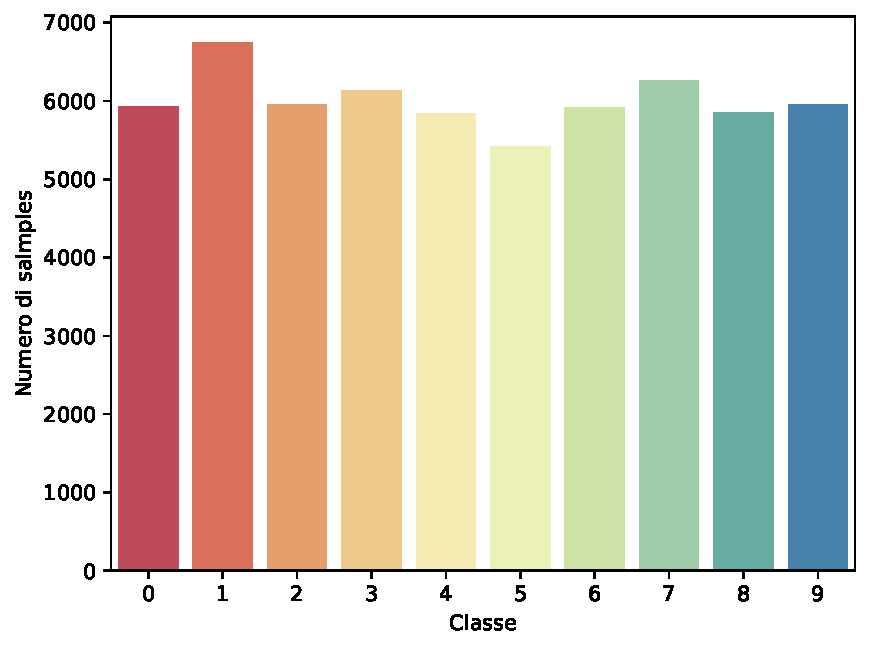
\includegraphics[width=\textwidth]{immages/2-analisi/distribuzione MNIST.pdf}
        \caption{MNIST}
    \end{subfigure}
    \hfill
    \begin{subfigure}{0.3\textwidth}
        \centering
        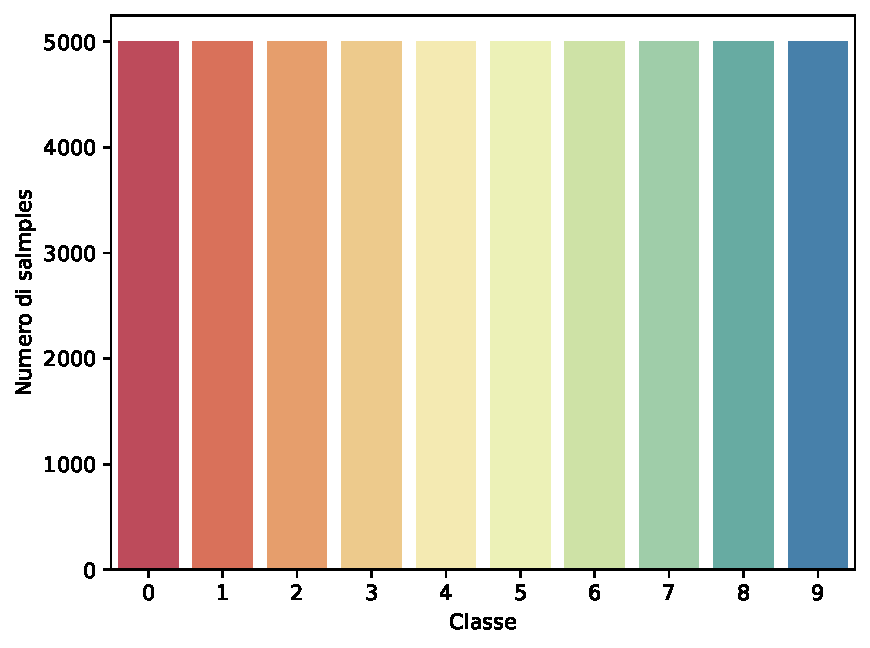
\includegraphics[width=\textwidth]{immages/2-analisi/distribuzione CIFAR10.pdf}
        \caption{CIFAR-10}
    \end{subfigure}
    \hfill
    \begin{subfigure}{0.3\textwidth}
        \centering
        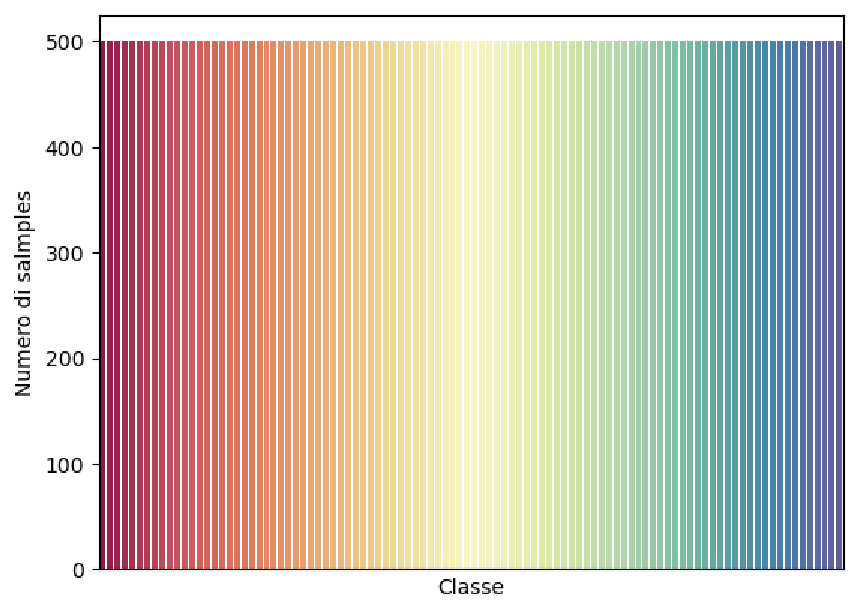
\includegraphics[width=\textwidth]{immages/2-analisi/distribuzione CIFAR100.pdf}
        \caption{CIFAR-100}
    \end{subfigure}
    \caption{Distribuzione del train set}
    \label{fig:distribuzione}
\end{figure}

%%%%%%%%%%%%%%%%%%%%%%%%%%%%%%%%%%%%%%%%%%%%%%%%%%%%
\section{MNIST}
\label{sec:MNIST}
MNIST è un dataset relativamente semplice, i cui elementi rappresentano immagini di numeri scritti a mano. Il compito di classificazione sta nel decidere a quale delle possibili 10 classi appartiene un elemento. Ogni istanza ha una dimensione $28\times28$ con un solo canale in scala di grigi. Ogni pixel è un numero naturale da 0 a 255, dove 0 indica il nero e 255 il bianco. È composto da 70K samples totali, già divisi in un train set da 60K samples e un test set da 10K.

Per rappresentare la sua semplicità (soprattutto rispetto a CIFAR-10), si sono rappresentati i dati in due dimensioni tramite l'algoritmo t-SNE, come si vede in Figura \ref{fig:raggruppamentoMNIST}.

Durante l'importazione, gli elementi del dataset sono stati trasformati in tensori e normalizzati usando la media e la varianza.

\begin{figure}[htbp]
    \centering
    \begin{subfigure}{0.45\textwidth}
        \centering
        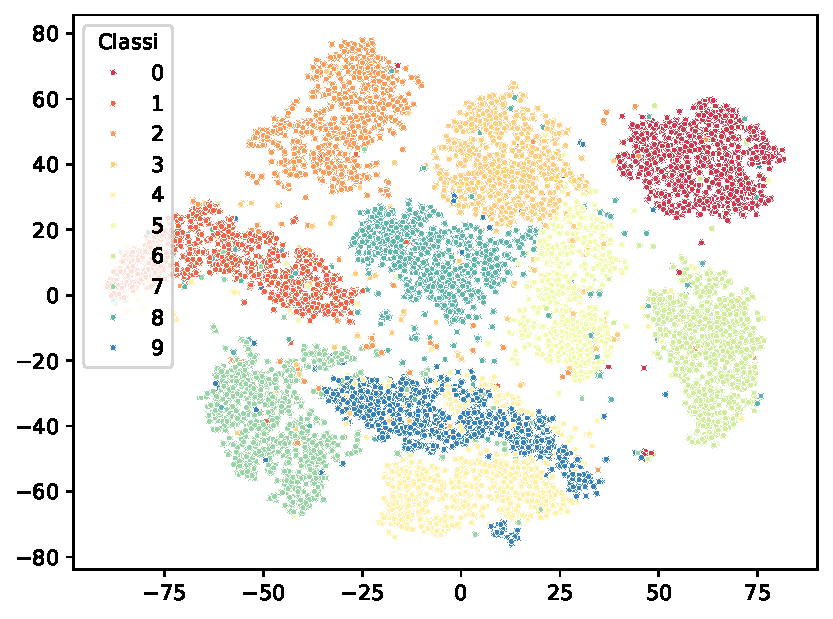
\includegraphics[width=\textwidth]{immages/2-analisi/raggruppamento MNIST.pdf}
        \caption{MNIST}
        \label{fig:raggruppamentoMNIST}
    \end{subfigure}
    \hfill
    \begin{subfigure}{0.45\textwidth}
        \centering
        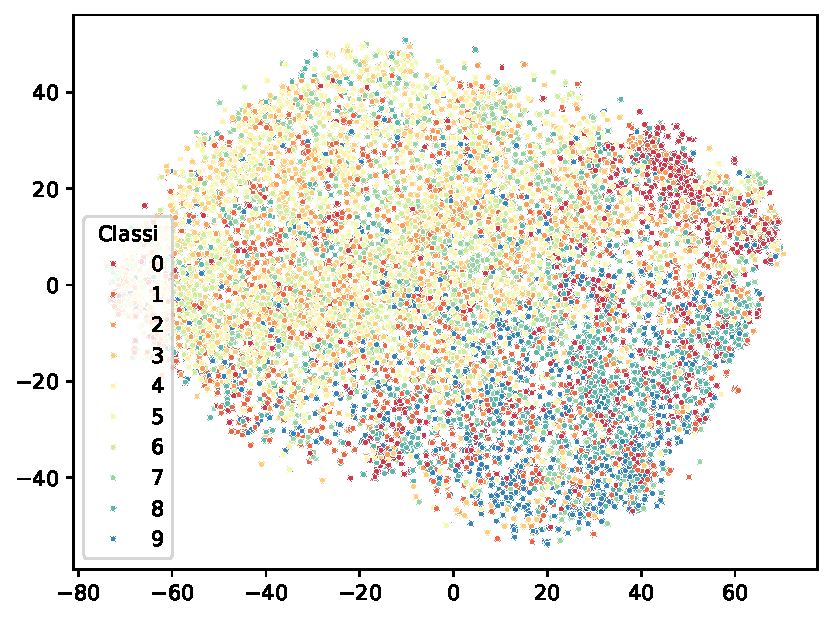
\includegraphics[width=\textwidth]{immages/2-analisi/raggruppamento CIFAR10.pdf}
        \caption{CIFAR-10}
        \label{fig:raggruppamentoCIFAR10}
    \end{subfigure}
    \caption{t-SNE in due dimensioni MNIST e CIFAR-10}
\end{figure}

%%%%%%%%%%%%%%%%%%%%%%%%%%%%%%%%%%%%%%%%%%%%%%%%%%%%
\section{CIFAR-10}
\label{sec:CIFAR10}
CIFAR-10 è un dataset più complesso rispetto a MNIST, i cui elementi rappresentano immagini di oggetti. Il compito di classificazione, anche in questo caso, è quello di predire una delle possibili 10 classi. Ogni elemento del dataset è un'immagine $32\times32$ con tre canali, come mostrato in Figura \ref{fig:esempioCIFAR10}; è quindi un'immagine RGB, dove per ogni canale 0 rappresenta il nero e 255 il bianco. È composto da 60K samples totali, dove 50K sono dedicati al train set e 10K al test set. Il test set è perfettamente bilanciato con 5K immagini per classe.

Anche in questo caso, per mettere in evidenza la difficoltà della classificazione rispetto a MNIST, si è usato t-SNE su due dimensioni, come si vede in Figura \ref{fig:raggruppamentoCIFAR10}.

Durante l'importazione, oltre alle operazioni eseguite per MNIST, i dati sono stati anche scalati in $128\times128$. In questo modo si sono potute eseguire più di 3 operazioni di pooling (supponendo di dimezzare la dimensionalità ad ogni operazione).

\begin{figure}[htbp]
    \centering
    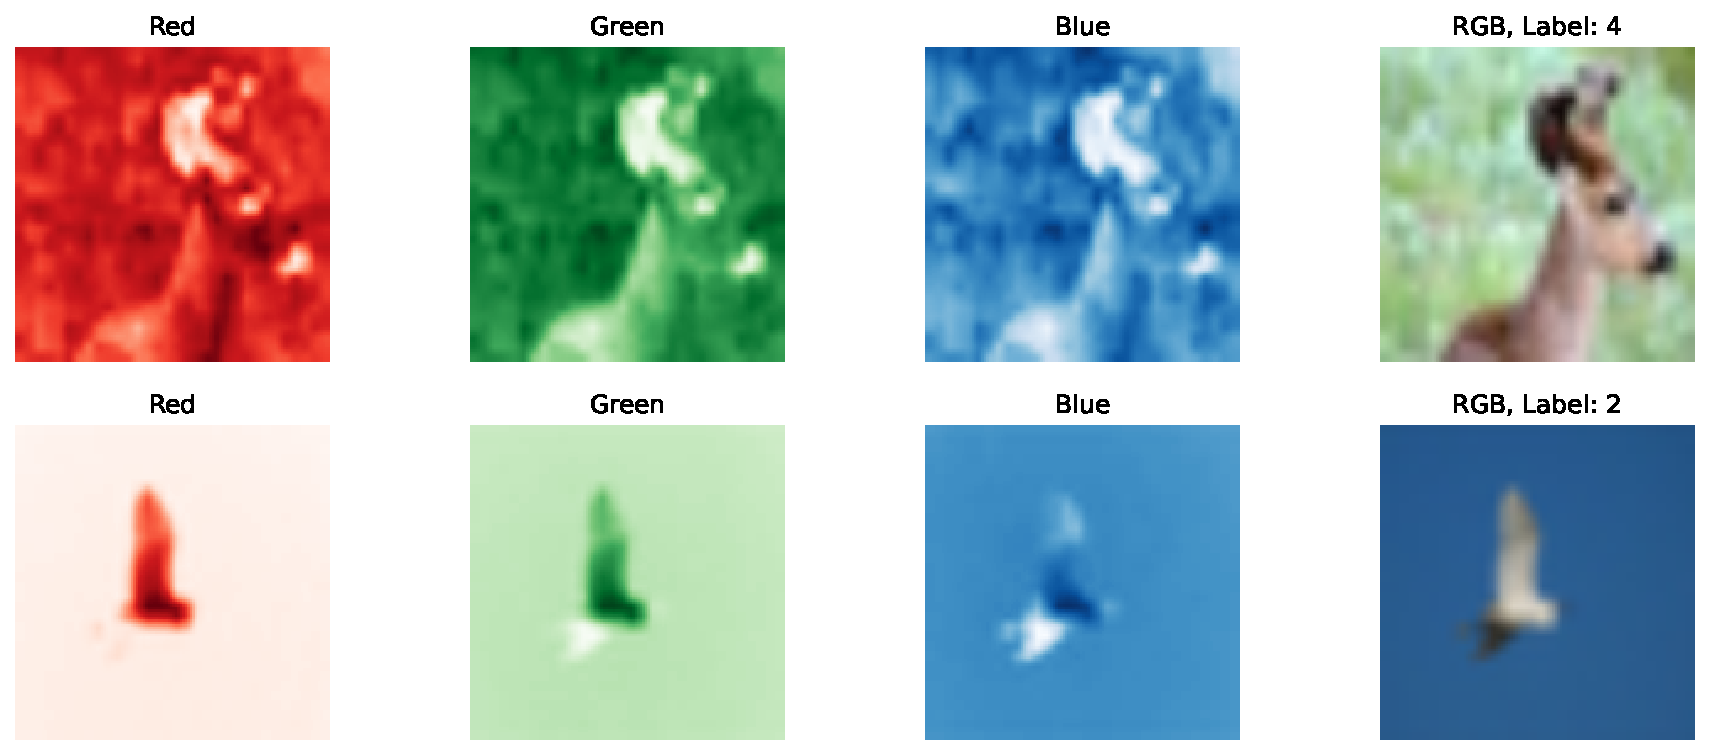
\includegraphics[width=0.6\textwidth]{immages/2-analisi/immagini CIFAR10.pdf}
    \caption{Esempio CIFAR-10 RGB}
    \label{fig:esempioCIFAR10}
\end{figure}

%%%%%%%%%%%%%%%%%%%%%%%%%%%%%%%%%%%%%%%%%%%%%%%%%%%%
\section{CIFAR-100}
\label{sec:CIFAR100}
CIFAR-100 ha esattamente la stessa struttura di CIFAR-10 (Figura \ref{fig:esempioCIFAR100}), ma con piccole e sostanziali differenze che rendono più complesso il lavoro di predizione (Figura \ref{fig:raggruppamentoCIFAR}) \cite{cifar}:

\begin{enumerate}
    \item Le classi sono gerarchiche. Abbiamo 20 super classi, ognuna delle quali è raffinata in 5 sotto-classi, per un totale di 100 classi.
    \item Siccome il numero di samples è lo stesso, ci sono poche immagini per ogni classe. In particolare, per ogni classe, ci sono 500 immagini per il train set e 100 per il test set.
\end{enumerate}

Come in CIFAR-10, il formato delle immagini è sempre $32\times32\times3$ (RGB). Queste sono state scalate a $128\times128$ per gli stessi motivi elencati sopra.

\begin{figure}[htbp]
    \centering
    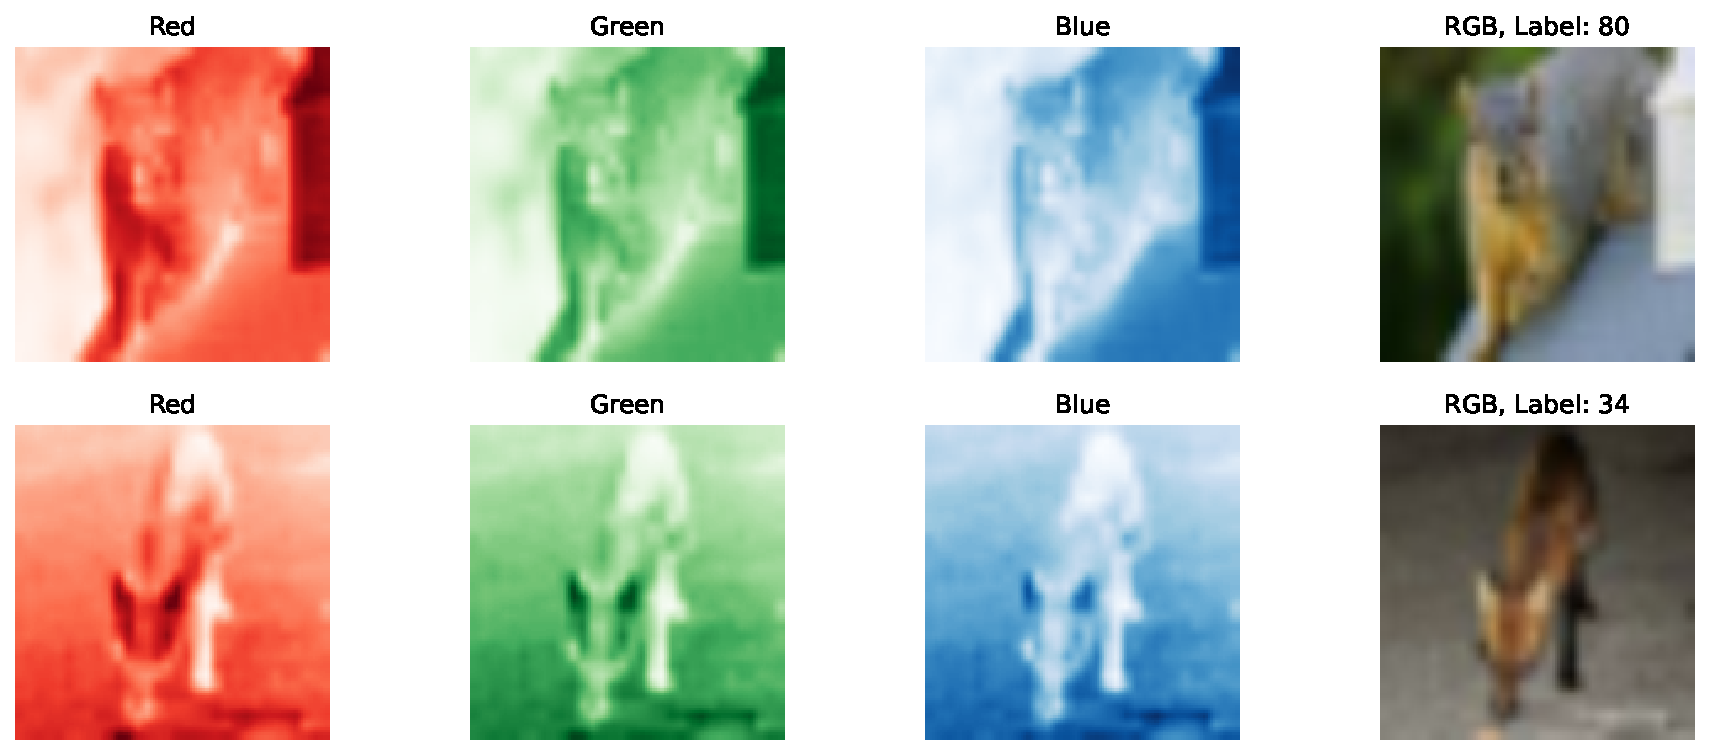
\includegraphics[width=0.6\textwidth]{immages/2-analisi/immagini CIFAR100.pdf}
    \caption{Esempio CIFAR-100 RGB}
    \label{fig:esempioCIFAR100}
\end{figure}

\begin{figure}[htbp]
    \centering
    \begin{subfigure}{0.45\textwidth}
        \centering
        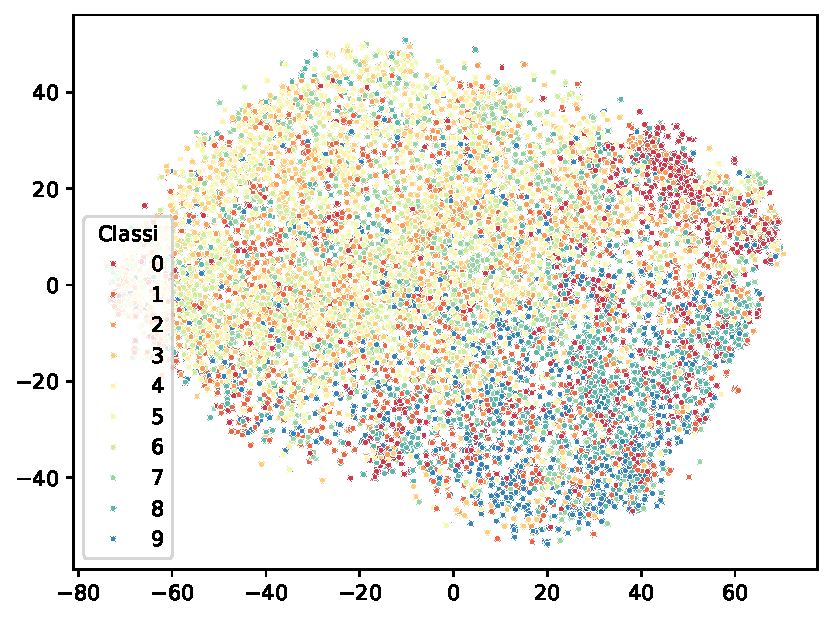
\includegraphics[width=\textwidth]{immages/2-analisi/raggruppamento CIFAR10.pdf}
        \caption{CIFAR-10}
    \end{subfigure}
    \hfill
    \begin{subfigure}{0.45\textwidth}
        \centering
        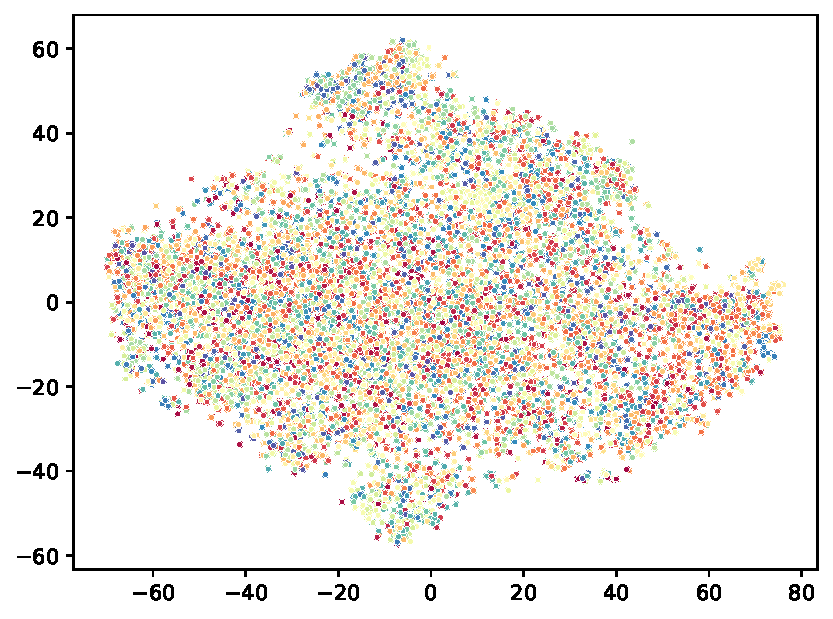
\includegraphics[width=\textwidth]{immages/2-analisi/raggruppamento CIFAR100.pdf}
        \caption{CIFAR-100}
    \end{subfigure}
    \caption{t-SNE in due dimensioni CIFAR-10 e CIFAR-100}
    \label{fig:raggruppamentoCIFAR}
\end{figure}